\section{Method}
% What to add:
% 
% Show and explain the cituit made and choices of components
The metal detector is made up of three parts: the oscillator, the transformer and the rectifier.
As for the oscillator a colpitts oscillator was chosen for its simplicity and since the required components were available. 
A 10 mH inductor and two 3.3 uF capacitors were used for the LC circuit and the OP-amp increased the signal by 5 times.

The Transformer was made using two coils which were then zip tied together. The resistor between the coil connected to the oscillator 
and ground had a variable resistor to allow for the the signal to be tuned. A lowered resistance results in a stronger signal
 being induced in the second coil, but also in a less stable oscillation. The signal from the second coil was then amplified 10 times to make
 it stronger.

Finally the rectifier chosen was a  half-wave rectifier using a single diode and a capacitor which would allow for the signal to more 
easily be detected either by eye or a seperate system.

\begin{figure}[h]
    \centering
    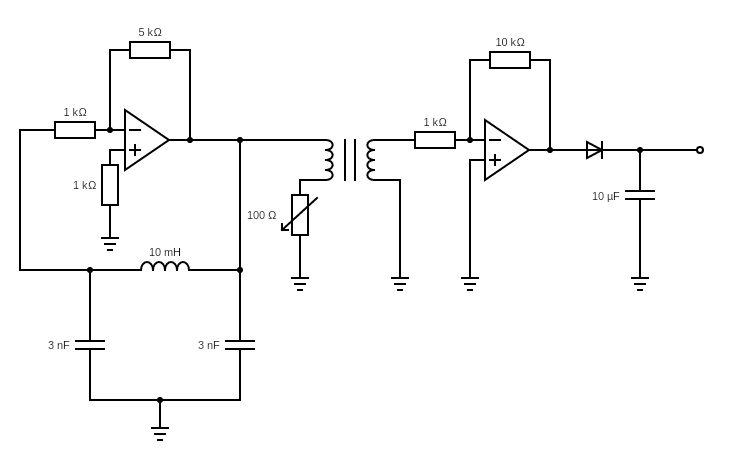
\includegraphics[scale=0.60]{circuit.png}
    \caption{A diagram of the circuit of the metal detector discussed in this report}
    \label{fig:rnn_basic}
\end{figure}